\section{Durchführung}
\label{sec:Durchführung}

\subsection{Messen der Falldauern der Kugeln im Viskosimeter}
Beim Kugelfallviskosimeter nach Höppler (Abb. \ref{fig:viskosimeter}) wird die Kugel in einem Rohr, 
dessen Radius nur geringfügig größer ist als der Radius der Kugel, fallen gelassen.
Mithilfe der Libelle wird das Viskosimeter justiert, falls es nicht gerade steht.
\begin{figure}
    \centering
    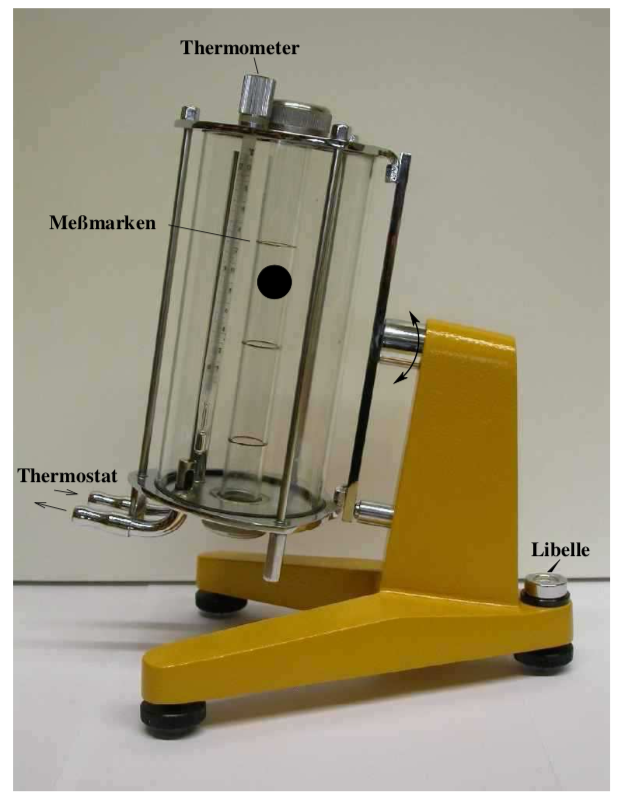
\includegraphics[width=10cm, height=10cm]{build/viskosimeter.png}
    \caption{Das Kugelfall-Viskosimeter nach Höppler.
    In dem Rohr im Inneren des Wasserbads befindet sich destilliertes Wasser.
    Die Kugel wird in dem Rohr fallen gelassen. Durch das Thermostat kann die 
    Temperatur des Wasserbads eingestellt werden.}
    \label{fig:viskosimeter}
\end{figure}
\noindent Das Viskosimeter wird mit destilliertem Wasser gefüllt, wobei darauf geachtet wird, 
dass sich keine Luftblasen an der Rohrwand oder an der Kugel befinden. 
Da beim senkrechten Fall Wirbel entstehen könnten und die Kugel unkontrolliert an die 
Rohrwand stoßen würde, wird das Fallrohr um einen kleinen Winkel gekippt.
Die Kugel kann an der Rohrwand heruntergleiten.
\newline
Zunächst wird die Dichte der großen und kleinen Glaskugel aus der Masse und dem Volumen bestimmt.  
Anschließend werden jeweils zehn Fallzeiten für die kleine und die große Kugel bei Raumtemperatur 
mit einer Stoppuhr gemessen. Es wird die Zeit gemessen, die die Kugel nach Überschreiten der ersten Markierung
bis zum Überschreiten der letzten Markierung braucht.
Wenn die Kugel die untere Markierung überschreitet, 
wird das Viskosimeter um $\SI{180}{\degree}$ gedreht und die Messung wiederholt.  
% Somit wird für die große Kugel die Apparaturkonstante $K_{gr}$ bestimmt. 
% Die Apparaturkonstante für die kleine Kugel ist bereits gegeben. 

\subsection{Messen der Temperaturabhängigkeit der Viskosität von destilliertem Wasser}
Als nächstes wird die Temperaturabhängigkeit von destilliertem Wasser bestimmt. 
Dazu wird das Wasserbad auf $\SI{70}{\degree}$ aufgeheizt. Die Fallzeit der großen Kugel wird jeweils zwei mal 
für zehn verschiedene Temperaturen gemessen.